\documentclass[11pt,letterpaper]{article}
\usepackage[margin=0.85in,headheight=14pt]{geometry}
\usepackage{amsmath,amssymb}
\usepackage{enumitem}
\usepackage{fancyhdr}
\usepackage{lmodern}
\usepackage[T1]{fontenc}
\usepackage[dvipsnames]{xcolor}
\usepackage[most]{tcolorbox}
\usepackage{pgfplots}
\usepgfplotslibrary{groupplots}
\pgfplotsset{
  compat=1.18,
  every axis/.append style={grid=major, grid style={gray!25}, tick label style={font=\footnotesize},
    label style={font=\small}, title style={font=\small}, legend style={font=\scriptsize}},
}
\definecolor{cA}{HTML}{1F77B4}
\definecolor{cB}{HTML}{FF7F0E}
\definecolor{cC}{HTML}{2CA02C}
\definecolor{cD}{HTML}{D62728}
\definecolor{cE}{HTML}{9467BD}

\pagestyle{fancy}
\fancyhf{}
\lhead{SYDE 556/750 \qquad Final practice}
\rhead{Solutions}
\cfoot{\thepage}
\renewcommand{\headrulewidth}{0pt}

\setlength{\parindent}{0pt}
\setlength{\parskip}{4pt}

\newcommand{\Jb}{J^{\mathrm{bias}}}
\newcommand{\T}{\mathsf T}
\newcommand{\ans}[1]{\par\vspace{4pt}{\bfseries #1}\quad}

\newtcolorbox{result}{colback=Green!6,colframe=Green!50!black,boxrule=0.5pt,left=4pt,right=4pt,top=2pt,bottom=2pt,arc=1pt}

\begin{document}

\begin{center}
{\Large\bfseries Final practice solutions}\\[2pt]
{\large Function decoders and filters}\\[4pt]
Open a solution only after attempting that question. Each green box is the result.
\end{center}

%---------------------------------------------------------------------
\section{Decoders from kinked tuning curves}

\ans{(a)}
Evaluate each neuron at $x = -1, 0, 1$:
\[
A = \begin{pmatrix} 0 & 0 & 1 \\ 1 & 0 & 0 \\ 0 & 1 & 2 \end{pmatrix}
\begin{matrix} \leftarrow a_1 \\ \leftarrow a_2 \\ \leftarrow a_3 \end{matrix}
\]
Neurons 1 and 2 bend at $x = 0$, inside the interval. Neuron 3 bends at $x = -1$, the edge, so on $[-1, 1]$ it is the straight line $x + 1$.
\begin{center}
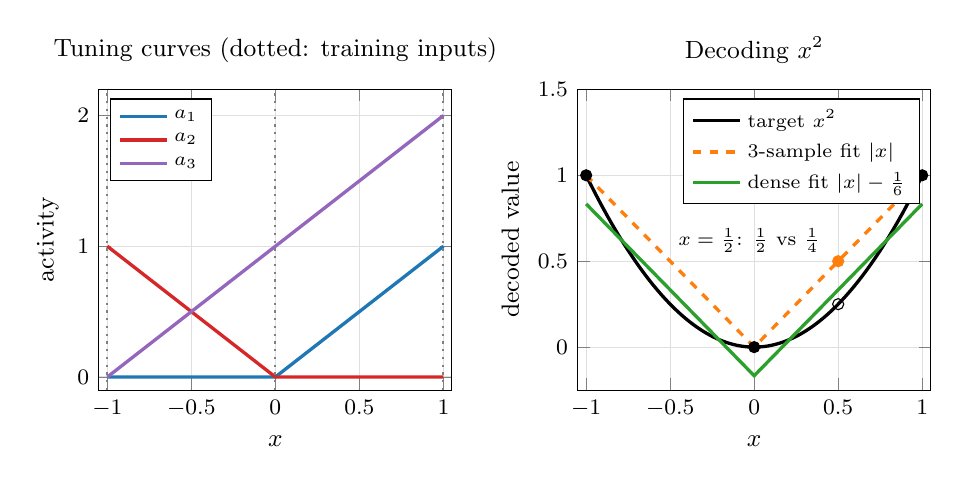
\begin{tikzpicture}
\begin{groupplot}[group style={group size=2 by 1, horizontal sep=1.6cm},
  width=0.5\textwidth, height=5.4cm, xmin=-1.05, xmax=1.05, xlabel={$x$}]
\nextgroupplot[title={Tuning curves (dotted: training inputs)}, ylabel={activity},
  legend pos=north west, ymin=-0.1, ymax=2.2]
  \addplot[cA, very thick, domain=-1:1, samples=201] {max(x,0)};
  \addplot[cD, very thick, domain=-1:1, samples=201] {max(-x,0)};
  \addplot[cE, very thick, domain=-1:1, samples=3] {x+1};
  \legend{$a_1$, $a_2$, $a_3$}
  \draw[gray, dotted, thick] (axis cs:-1,-0.1) -- (axis cs:-1,2.2);
  \draw[gray, dotted, thick] (axis cs:0,-0.1) -- (axis cs:0,2.2);
  \draw[gray, dotted, thick] (axis cs:1,-0.1) -- (axis cs:1,2.2);
\nextgroupplot[title={Decoding $x^2$}, ylabel={decoded value}, ymin=-0.25, ymax=1.5,
  legend pos=north east, legend cell align=left]
  \addplot[black, very thick, domain=-1:1, samples=201] {x^2};
  \addplot[cB, very thick, dashed, domain=-1:1, samples=201] {abs(x)};
  \addplot[cC, very thick, domain=-1:1, samples=201] {abs(x)-1/6};
  \legend{target $x^2$, 3-sample fit $|x|$, dense fit $|x|-\frac16$}
  \addplot[only marks, mark=*, black] coordinates {(-1,1) (0,0) (1,1)};
  \addplot[only marks, mark=*, cB] coordinates {(0.5,0.5)};
  \addplot[only marks, mark=o, black, mark options={fill=white}] coordinates {(0.5,0.25)};
  \node[font=\scriptsize, anchor=east] at (axis cs:0.45,0.62) {$x=\frac12$: $\frac12$ vs $\frac14$};
\end{groupplot}
\end{tikzpicture}
\end{center}
The left panel is the sketch. The right panel is for parts (d) and (e).

\ans{(b)}
Read the columns of $A$. At $x = -1$ the rates are $(0, 1, 0)$, at $x = 0$ they are $(0, 0, 1)$, at $x = 1$ they are $(1, 0, 2)$. With decoder $(p, q, r)$ the decoded values at the three samples are
\[
q, \qquad r, \qquad p + 2r .
\]
So matching a target $f$ means $q = f(-1)$, \ $r = f(0)$, \ $p = f(1) - 2f(0)$.
\[
f = x:\ (1, -1, 0), \qquad f = |x|:\ (1, 1, 0), \qquad f = 1:\ (-1, 1, 1).
\]
$A$ is square and invertible, so an exact match exists and is unique. Least squares with zero residual must return it: $(AA^\T)^{-1} A F^\T = A^{-\T} F^\T$.
\begin{result}
$D^{x} = (1, -1, 0)$, \ $D^{|x|} = (1, 1, 0)$, \ $D^{\mathbf 1} = (-1, 1, 1)$.
\end{result}

\ans{(c)}
The decoder is linear in the target, so $D^{3x - 2} = 3D^x - 2D^{\mathbf 1}$:
\[
3(1, -1, 0) - 2(-1, 1, 1) = (5, -5, -2).
\]
At $x = 1/2$ the rates are $(1/2,\ 0,\ 3/2)$, so $\hat y = 5/2 - 0 - 3 = -1/2$, and $3(1/2) - 2 = -1/2$.
\begin{result}
$D^{3x-2} = (5, -5, -2)$. It gives $-1/2$ at $x = 1/2$, matching.
\end{result}

\ans{(d)}
At the samples $x^2 = (1, 0, 1)$, which is exactly $|x|$ at the samples. So the decoder is $(1, 1, 0)$ again. At $x = 1/2$ it decodes $|1/2| = 1/2$, but $(1/2)^2 = 1/4$.

Three samples cannot tell $x^2$ from $|x|$. The decoder only fits where it was trained. That is why decoders are fitted over many samples covering the domain, not just a few points.
\begin{result}
$(1, 1, 0)$, decoding $1/2$ instead of $1/4$ at $x = 1/2$: too few samples.
\end{result}

\ans{(e)}
On $[-1, 1]$, \ $a_1 - a_2 = x$, \ $a_1 + a_2 = |x|$, \ $a_3 = x + 1$. So
\[
p a_1 + q a_2 + r a_3 = r + \Big(\tfrac{p - q}{2} + r\Big) x + \tfrac{p + q}{2}\,|x| = c_0 + c_1 x + c_2|x| .
\]
Every decoder gives a V shape with its corner at $0$. It can never curve.

Fit $c_0 + c_2 x$ to $x^2$ on $[0, 1]$. Set the error orthogonal to $1$ and to $x$:
\[
\int_0^1 (x^2 - c_0 - c_2 x)\,dx = \tfrac13 - c_0 - \tfrac{c_2}{2} = 0, \qquad
\int_0^1 (x^2 - c_0 - c_2 x)\,x\,dx = \tfrac14 - \tfrac{c_0}{2} - \tfrac{c_2}{3} = 0 .
\]
The first gives $c_0 = 1/3 - c_2/2$. Substituting, $1/12 - c_2/12 = 0$, so $c_2 = 1$ and $c_0 = -1/6$. The fit is $|x| - 1/6$.

As a decoder, $D^{|x|} - \tfrac16 D^{\mathbf 1} = (1, 1, 0) - \tfrac16(-1, 1, 1) = (7/6,\ 5/6,\ -1/6)$. Check: $c_0 = r = -1/6$, $c_1 = 1/6 - 1/6 = 0$, $c_2 = 1$.

Error $x^2 - (|x| - 1/6)$: \ $+1/6$ at $x = 0$ and at $x = \pm 1$, \ $-1/12$ at $x = \pm 1/2$. The fit shifts down so that it misses a little everywhere instead of a lot in the middle (green curve, right panel). More neurons with kinks spread across the interval would let the decoded curve bend.
\begin{result}
Dense fit $|x| - 1/6$, decoder $(7/6,\ 5/6,\ -1/6)$. Largest error $1/6$, at $x = 0$ and $x = \pm1$.
\end{result}

%---------------------------------------------------------------------
\section{What the noise penalty buys}

\ans{(a)}
With one neuron, $AA^\T = 1^2 + 2^2 = 5$ and $AX^\T = 1\cdot 1 + 2 \cdot 2 = 5$. So $d = 5/5 = 1$, and the decoded values are $(1, 2)$, exact.

\ans{(b)}
$d = AX^\T / (AA^\T + N\sigma^2) = 5 / (5 + 2 \cdot 2.5) = 1/2$. Decoded values $(1/2,\ 1)$. The decoder shrank toward zero, so clean reconstructions are now too small.
\begin{result}
$d = 1$ unregularized; $d = 1/2$ with $\sigma^2 = 2.5$.
\end{result}

\ans{(c)}
\[
E(d) = \tfrac12\big[(d - 1)^2 + (2d - 2)^2\big] + d^2\sigma^2 = \tfrac52 (d - 1)^2 + 2.5\, d^2 .
\]
$E(1) = 0 + 2.5 = 2.5$. \quad $E(1/2) = \tfrac52\cdot\tfrac14 + 2.5\cdot\tfrac14 = 0.625 + 0.625 = 1.25$.

The regularized decoder is worse on clean data but half the total error on noisy data.

\ans{(d)}
$dE/dd = 5(d - 1) + 5d = 0$ gives $d = 1/2$, the decoder from (b). This is what the $N\sigma^2$ term is for: the regularized formula minimizes clean error plus the noise each coefficient amplifies.
\begin{center}
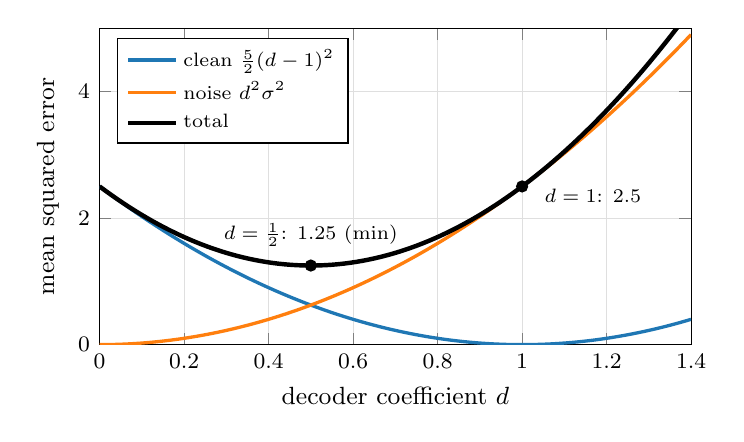
\begin{tikzpicture}
\begin{axis}[width=0.75\textwidth, height=5.6cm, xmin=0, xmax=1.4, ymin=0, ymax=5,
  xlabel={decoder coefficient $d$}, ylabel={mean squared error}, legend pos=north west,
  legend cell align=left]
  \addplot[cA, very thick, domain=0:1.4, samples=100] {2.5*(x-1)^2};
  \addplot[cB, very thick, domain=0:1.4, samples=100] {2.5*x^2};
  \addplot[black, ultra thick, domain=0:1.4, samples=100] {2.5*(x-1)^2 + 2.5*x^2};
  \legend{clean $\frac52(d-1)^2$, noise $d^2\sigma^2$, total}
  \addplot[only marks, mark=*, black] coordinates {(0.5,1.25) (1,2.5)};
  \node[font=\scriptsize, anchor=south] at (axis cs:0.5,1.4) {$d=\frac12$: 1.25 (min)};
  \node[font=\scriptsize, anchor=west] at (axis cs:1.03,2.35) {$d=1$: 2.5};
\end{axis}
\end{tikzpicture}
\end{center}
\begin{result}
$E(1) = 2.5$, \ $E(1/2) = 1.25$. The minimizer is $d = 1/2$.
\end{result}

%---------------------------------------------------------------------
\section{A two-dimensional function, then weights}

\ans{(a)}
Stack one decoder row per output component:
\[
D^f = \begin{pmatrix} D^x \\ D^{|x|} \end{pmatrix} = \begin{pmatrix} 1 & -1 & 0 \\ 1 & 1 & 0 \end{pmatrix}, \qquad 2 \times 3 .
\]

\ans{(b)}
Row $i$ of $E$ is $\alpha_i e_i^\T$:
\[
E = \begin{pmatrix} 2 & 0 \\ 0 & 1 \\ -3 & 0 \end{pmatrix}\ (3 \times 2), \qquad
W^f = E D^f = \begin{pmatrix} 2 & -2 & 0 \\ 1 & 1 & 0 \\ -3 & 3 & 0 \end{pmatrix}\ (3 \times 3).
\]
Row 1 is $2\times$ the $x$ decoder, row 2 is the $|x|$ decoder, row 3 is $-3\times$ the $x$ decoder. Each B neuron only reads the component its encoder points at.

\ans{(c)}
Column 3 is zero. Neuron 3 is the only one with a constant offset, and neither $x$ nor $|x|$ needs a constant. Neurons 1 and 2 already build both functions, so its decoder coefficient is zero in both rows.

\ans{(d)}
At $x = -1$ the rates are $a = (0, 1, 0)$, so $W^f a$ is column 2:
\[
J = \begin{pmatrix} -2 \\ 1 \\ 3 \end{pmatrix} + \begin{pmatrix} 1/2 \\ 1 \\ 0 \end{pmatrix} = \begin{pmatrix} -3/2 \\ 2 \\ 3 \end{pmatrix}.
\]
With the true $y = (-1, 1)$: \ $J_1 = 2(-1) + 1/2 = -3/2$, \ $J_2 = 1(1) + 1 = 2$, \ $J_3 = 3(-1)(-1) + 0 = 3$. Same currents.

\ans{(e)}
Column 1 is $(2, 1, -3)$ and column 2 is $(-2, 1, 3)$. Both mix signs, so pre-neurons 1 and 2 violate Dale's principle. Pre-neuron 3 has no connections.
\begin{result}
$W^f = \begin{pmatrix} 2 & -2 & 0 \\ 1 & 1 & 0 \\ -3 & 3 & 0 \end{pmatrix}$. \ At $x = -1$, $J = (-3/2,\ 2,\ 3)$ by both routes.
\end{result}

%---------------------------------------------------------------------
\section{An exponential synapse on a regular spike train}

\ans{(a)}
Each spike adds a jump of $1/\tau = 200\ \mathrm{s^{-1}}$ that then decays by $e^{-1}$ every 5 ms.
\[
s(10^-) = 200(e^{-2} + e^{-1}) = 200(0.503) \approx 100.6\ \mathrm{s^{-1}}, \qquad s(10^+) = 100.6 + 200 = 300.6\ \mathrm{s^{-1}},
\]
\[
s(15^-) = 200(e^{-3} + e^{-2} + e^{-1}) = 200(0.553) \approx 110.6\ \mathrm{s^{-1}} .
\]
\begin{center}
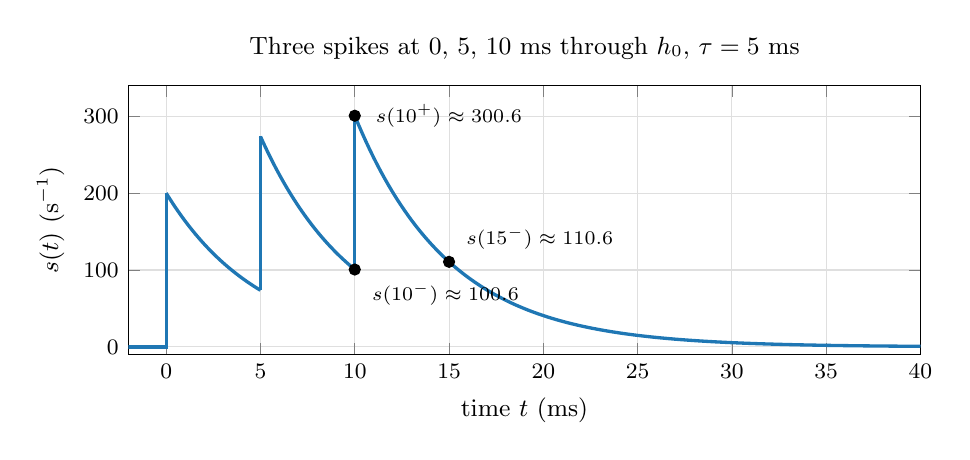
\begin{tikzpicture}
\begin{axis}[width=0.96\textwidth, height=5cm, xmin=-2, xmax=40, ymin=-10, ymax=340,
  xlabel={time $t$ (ms)}, ylabel={$s(t)$ (s$^{-1}$)},
  title={Three spikes at 0, 5, 10 ms through $h_0$, $\tau = 5$ ms}]
  \addplot[cA, very thick] coordinates {(-2,0) (0,0) (0,200)};
  \addplot[cA, very thick, domain=0:5, samples=40] {200*exp(-x/5)};
  \addplot[cA, very thick, domain=5:10, samples=40] {200*(exp(-x/5)+exp(-(x-5)/5))};
  \addplot[cA, very thick, domain=10:40, samples=150] {200*(exp(-x/5)+exp(-(x-5)/5)+exp(-(x-10)/5))};
  \draw[cA, very thick] (axis cs:5,73.6) -- (axis cs:5,273.6);
  \draw[cA, very thick] (axis cs:10,100.6) -- (axis cs:10,300.6);
  \addplot[only marks, mark=*, black] coordinates {(10,100.6) (10,300.6) (15,110.6)};
  \node[font=\scriptsize, anchor=west] at (axis cs:10.6,300.6) {$s(10^+) \approx 300.6$};
  \node[font=\scriptsize, anchor=north west] at (axis cs:10.4,96) {$s(10^-) \approx 100.6$};
  \node[font=\scriptsize, anchor=south west] at (axis cs:15.4,114) {$s(15^-) \approx 110.6$};
\end{axis}
\end{tikzpicture}

\vspace{4pt}
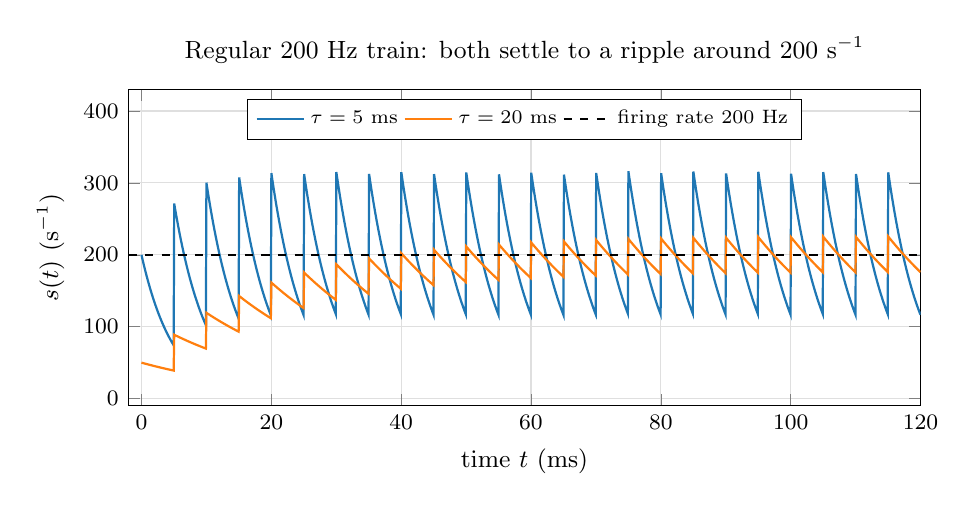
\begin{tikzpicture}
\begin{axis}[width=0.96\textwidth, height=5.6cm, xmin=-2, xmax=120, ymin=-10, ymax=430,
  xlabel={time $t$ (ms)}, ylabel={$s(t)$ (s$^{-1}$)},
  legend style={at={(0.5,0.97)}, anchor=north, legend columns=3},
  title={Regular 200 Hz train: both settle to a ripple around 200 s$^{-1}$}]
  \addplot[cA, thick, domain=0:119.99, samples=1500]
    {200*exp(-(x-5*floor(x/5))/5)*(1-exp(-(floor(x/5)+1)))/(1-exp(-1))};
  \addplot[cB, thick, domain=0:119.99, samples=1500]
    {50*exp(-(x-5*floor(x/5))/20)*(1-exp(-(floor(x/5)+1)/4))/(1-exp(-1/4))};
  \addplot[black, dashed, thick, domain=-2:120, samples=2] {200};
  \legend{$\tau = 5$ ms, $\tau = 20$ ms, firing rate 200 Hz}
\end{axis}
\end{tikzpicture}
\end{center}

\ans{(b)}
$P(1 - e^{-T/\tau}) = 1/\tau$, so with $T/\tau = 1$:
\[
P = \frac{200}{1 - 0.368} \approx 316\ \mathrm{s^{-1}}, \qquad \text{trough} = P e^{-1} \approx 116\ \mathrm{s^{-1}} .
\]

\ans{(c)}
\[
\frac1T \int_0^T P e^{-t/\tau}\,dt = \frac{P\tau}{T}\big(1 - e^{-T/\tau}\big) = \frac{\tau}{T}\cdot\frac{1}{\tau} = \frac1T = 200\ \mathrm{s^{-1}} .
\]
Unit area: every spike contributes exactly one unit of area, so the average filtered activity is the spike count per second, the firing rate.

\ans{(d)}
With $\tau = 20$ ms, $1/\tau = 50\ \mathrm{s^{-1}}$ and $e^{-T/\tau} = e^{-0.25} \approx 0.779$:
\[
P = \frac{50}{0.221} \approx 226\ \mathrm{s^{-1}}, \qquad \text{trough} \approx 226 \cdot 0.779 \approx 176\ \mathrm{s^{-1}} .
\]
The ripple is always the jump $1/\tau$: $200\ \mathrm{s^{-1}}$ at $\tau = 5$ ms, $50\ \mathrm{s^{-1}}$ at $\tau = 20$ ms. The mean is $200\ \mathrm{s^{-1}}$ for both. Decoded with $d = 0.004$: mean $0.8$ for both, ripple $0.8$ versus $0.2$.

The cost: the larger $\tau$ takes several $\tau$ to settle (bottom panel, the orange trace takes about 60 ms) and lags or attenuates any fast change in the rate.
\begin{result}
$s(10^\pm) \approx 100.6,\ 300.6\ \mathrm{s^{-1}}$, \ $s(15^-) \approx 110.6\ \mathrm{s^{-1}}$. \ Steady state: $316/116$ at $\tau = 5$ ms, $226/176$ at $\tau = 20$ ms, both averaging $200\ \mathrm{s^{-1}}$.
\end{result}

%---------------------------------------------------------------------
\section{Two synapses with the same delay}

\ans{(a)}
Mean delay $(n+1)\tau$: filter A gives $1 \cdot 10 = 10$ ms, filter B gives $2 \cdot 5 = 10$ ms.

\ans{(b)}
At 10 Hz, $\omega \approx 62.8$ rad/s:
\[
|H_A| = \frac{1}{\sqrt{1 + 0.628^2}} = \frac{1}{\sqrt{1.394}} \approx 0.847, \qquad
|H_B| = \frac{1}{1 + 0.314^2} = \frac{1}{1.0986} \approx 0.910 .
\]
At 100 Hz, $\omega \approx 628$ rad/s:
\[
|H_A| = \frac{1}{\sqrt{1 + 6.28^2}} = \frac{1}{\sqrt{40.4}} \approx 0.157, \qquad
|H_B| = \frac{1}{1 + 3.14^2} = \frac{1}{10.86} \approx 0.092 .
\]

\ans{(c)}
Filter B passes more of the 10 Hz signal and less of the 100 Hz noise, at the same mean delay. Its gain falls twice as steeply at high frequency (squared denominator).

The cost is at the start: $h_1(0) = 0$ and it peaks only at $t = \tau = 5$ ms, while $h_0$ responds at full height immediately. After a sudden change, filter B shows almost nothing for the first few milliseconds.
\begin{center}
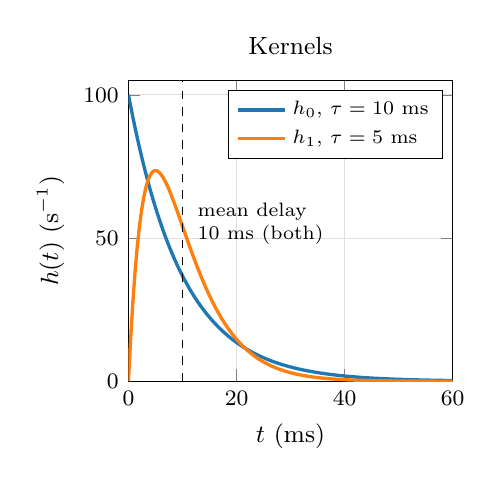
\begin{tikzpicture}
\begin{axis}[width=0.47\textwidth, height=5.4cm, xmin=0, xmax=60, ymin=0, ymax=105,
  xlabel={$t$ (ms)}, ylabel={$h(t)$ (s$^{-1}$)}, title={Kernels}, legend pos=north east,
  legend cell align=left]
  \addplot[cA, very thick, domain=0:60, samples=150] {100*exp(-x/10)};
  \addplot[cB, very thick, domain=0:60, samples=150] {40*x*exp(-x/5)};
  \legend{{$h_0$, $\tau=10$ ms}, {$h_1$, $\tau=5$ ms}}
  \draw[black, dashed] (axis cs:10,0) -- (axis cs:10,105);
  \node[font=\scriptsize, anchor=west, align=left] at (axis cs:11,55) {mean delay\\10 ms (both)};
\end{axis}
\end{tikzpicture}\hfill
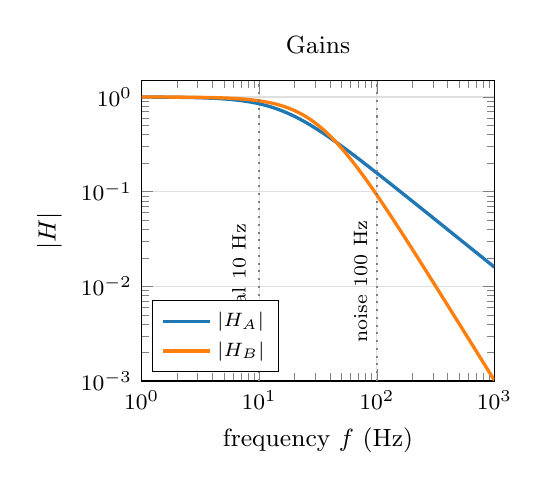
\begin{tikzpicture}
\begin{loglogaxis}[width=0.5\textwidth, height=5.4cm, xmin=1, xmax=1000, ymin=1e-3, ymax=1.5,
  xlabel={frequency $f$ (Hz)}, ylabel={$|H|$}, title={Gains}, legend pos=south west,
  legend cell align=left]
  \addplot[cA, very thick, domain=1:1000, samples=200] {1/sqrt(1+(2*pi*x*0.01)^2)};
  \addplot[cB, very thick, domain=1:1000, samples=200] {1/(1+(2*pi*x*0.005)^2)};
  \legend{$|H_A|$, $|H_B|$}
  \draw[gray, dotted, thick] (axis cs:10,1e-3) -- (axis cs:10,1.5);
  \draw[gray, dotted, thick] (axis cs:100,1e-3) -- (axis cs:100,1.5);
  \node[font=\scriptsize, rotate=90, anchor=south west] at (axis cs:10,2e-3) {signal 10 Hz};
  \node[font=\scriptsize, rotate=90, anchor=south west] at (axis cs:100,2e-3) {noise 100 Hz};
\end{loglogaxis}
\end{tikzpicture}
\end{center}

\ans{(d)}
Spikes are narrow pulses. A delta has a flat spectrum, so a spike train has power at every frequency, regardless of how slowly the underlying rate changes.
\begin{result}
10 Hz: $0.847$ (A), $0.910$ (B). \ 100 Hz: $0.157$ (A), $0.092$ (B). B is better on both, but starts from zero.
\end{result}

%---------------------------------------------------------------------
\section{The optimal filter when the response is amplified}

\ans{(a)}
$R^* = gX^* + \eta^*$.
\[
\langle X R^* \rangle = g\langle |X|^2 \rangle + \langle X\eta^* \rangle = g S_X,
\]
\[
\langle |R|^2 \rangle = g^2 \langle |X|^2 \rangle + g\langle X\eta^* \rangle + g\langle \eta X^* \rangle + \langle |\eta|^2 \rangle = g^2 S_X + S_\eta .
\]
Both cross terms vanish because $\langle \eta X^* \rangle = \langle X \eta^* \rangle^* = 0$.
\[
H = \frac{g S_X}{g^2 S_X + S_\eta} .
\]

\ans{(b)}
$S_\eta \to 0$: \ $H \to 1/g$, which undoes the gain exactly. \ $S_X = 0$: \ $H = 0$, since there is nothing to recover at that frequency.

\ans{(c)}
In band, $H = g/(g^2 + 4)$: \ $g = 1$: $1/5 = 0.2$. \ $g = 2$: $2/8 = 0.25$. \ $g = 4$: $4/20 = 0.2$. Out of band, $H = 0$.

\ans{(d)}
$gH = g^2 S_X / (g^2 S_X + S_\eta)$: \ $0.2$, \ $0.5$, \ $0.8$.

$H$ also has to undo the gain, so it is not a measure of quality by itself. With $g = 1$ the response is mostly noise and the filter keeps only $20\%$ of the input. With $g = 4$ the response is mostly signal, and the filter's $0.2$ is just $1/g$ shrunk slightly, keeping $80\%$. The quantity that matters is the signal-to-noise ratio $g^2 S_X / S_\eta$.
\begin{center}
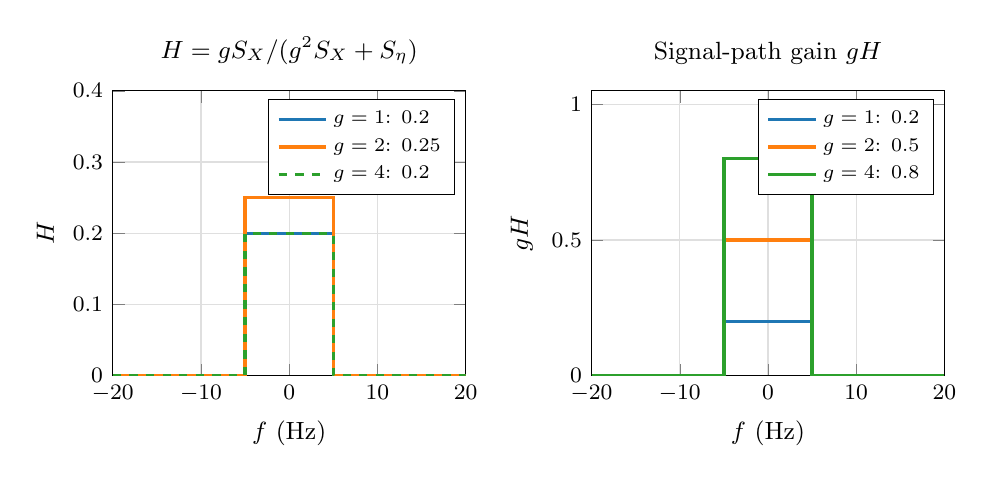
\begin{tikzpicture}
\begin{groupplot}[group style={group size=2 by 1, horizontal sep=1.6cm},
  width=0.5\textwidth, height=5.2cm, xmin=-20, xmax=20, xlabel={$f$ (Hz)},
  legend pos=north east, legend cell align=left]
\nextgroupplot[title={$H = gS_X/(g^2S_X+S_\eta)$}, ylabel={$H$}, ymin=0, ymax=0.4]
  \addplot[cA, very thick] coordinates {(-20,0) (-5,0) (-5,0.2) (5,0.2) (5,0) (20,0)};
  \addplot[cB, very thick] coordinates {(-20,0) (-5,0) (-5,0.25) (5,0.25) (5,0) (20,0)};
  \addplot[cC, very thick, dashed] coordinates {(-20,0) (-5,0) (-5,0.2) (5,0.2) (5,0) (20,0)};
  \legend{$g=1$: 0.2, $g=2$: 0.25, $g=4$: 0.2}
\nextgroupplot[title={Signal-path gain $gH$}, ylabel={$gH$}, ymin=0, ymax=1.05]
  \addplot[cA, very thick] coordinates {(-20,0) (-5,0) (-5,0.2) (5,0.2) (5,0) (20,0)};
  \addplot[cB, very thick] coordinates {(-20,0) (-5,0) (-5,0.5) (5,0.5) (5,0) (20,0)};
  \addplot[cC, very thick] coordinates {(-20,0) (-5,0) (-5,0.8) (5,0.8) (5,0) (20,0)};
  \legend{$g=1$: 0.2, $g=2$: 0.5, $g=4$: 0.8}
\end{groupplot}
\end{tikzpicture}
\end{center}
\begin{result}
$H = gS_X/(g^2S_X + S_\eta)$. \ In band $H = 0.2,\ 0.25,\ 0.2$ and $gH = 0.2,\ 0.5,\ 0.8$ for $g = 1, 2, 4$. Out of band $0$.
\end{result}

%---------------------------------------------------------------------
\section{Filter first or square first?}

\ans{(a)}
The decoded $x^2$ is a step from $0$ to $1$; one synapse turns it into $1 - e^{-t/\tau}$. At $t = \tau$: $1 - 0.368 = 0.632$.

\ans{(b)}
B represents $1 - e^{-t/\tau}$. Its $x^2$ decoder outputs $(1 - e^{-t/\tau})^2$. At $t = \tau$: $0.632^2 \approx 0.400$.

\ans{(c)}
The synapse is linear and squaring is not. Route 1 squares and then filters, $h * (x^2)$. Route 2 filters and then squares, $(h * x)^2$. These are different functions of time, though both end at $1$. They agree in steady state, or whenever $f$ is linear.

\ans{(d)}
At $t = \tau$: $1 - 2(0.368) - 0.135 \approx 0.129$. Ranking at $t = \tau$: Route 1 at C ($0.632$) $>$ Route 2 decoded by B ($0.400$) $>$ Route 2 at C ($0.129$).

\ans{(e)}
Route 1: $e^{-t/\tau} = 0.1$, so $t = \tau \ln 10 \approx 2.30\,\tau$. \
Route 2 at B: $1 - e^{-t/\tau} = \sqrt{0.9} \approx 0.949$, so $e^{-t/\tau} \approx 0.051$ and $t \approx 2.97\,\tau$. After the second synapse it takes about $4.5\,\tau$ (read from the plot).

Every extra population adds a synapse and slows the response. Computing a nonlinear function directly in one connection is faster than routing through an intermediate population.
\begin{center}
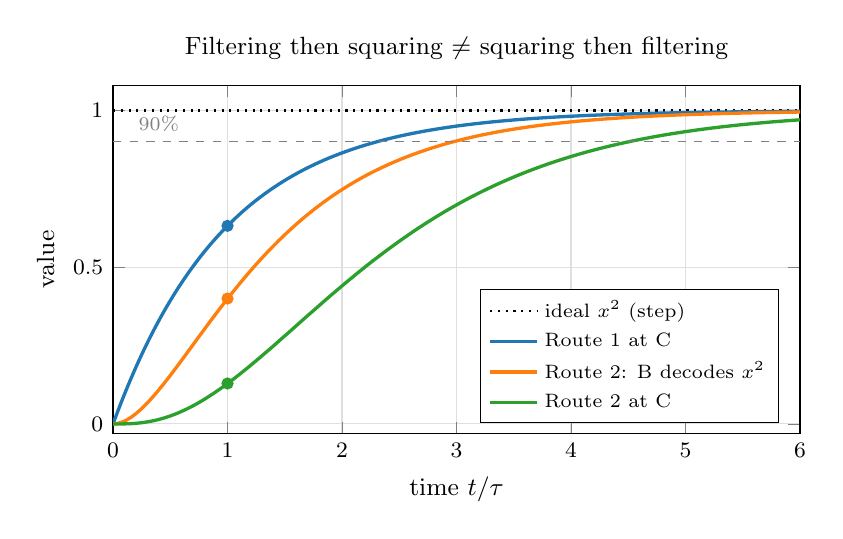
\begin{tikzpicture}
\begin{axis}[width=0.85\textwidth, height=6cm, xmin=0, xmax=6, ymin=-0.03, ymax=1.08,
  xlabel={time $t/\tau$}, ylabel={value}, legend pos=south east, legend cell align=left,
  title={Filtering then squaring $\neq$ squaring then filtering}]
  \addplot[black, dotted, thick, domain=0:6, samples=2] {1};
  \addplot[cA, very thick, domain=0:6, samples=150] {1-exp(-x)};
  \addplot[cB, very thick, domain=0:6, samples=150] {(1-exp(-x))^2};
  \addplot[cC, very thick, domain=0:6, samples=150] {1-2*x*exp(-x)-exp(-2*x)};
  \legend{ideal $x^2$ (step), Route 1 at C, Route 2: B decodes $x^2$, Route 2 at C}
  \addplot[gray, dashed, domain=0:6, samples=2, forget plot] {0.9};
  \node[font=\scriptsize, gray, anchor=south] at (axis cs:0.4,0.9) {90\%};
  \addplot[only marks, mark=*, cA, forget plot] coordinates {(1,0.632)};
  \addplot[only marks, mark=*, cB, forget plot] coordinates {(1,0.400)};
  \addplot[only marks, mark=*, cC, forget plot] coordinates {(1,0.129)};
\end{axis}
\end{tikzpicture}
\end{center}
\begin{result}
At $t = \tau$: $0.632$, $0.400$, $0.129$. \ $90\%$ times: $2.30\tau$ (Route 1), $2.97\tau$ (B's decoded $x^2$), about $4.5\tau$ (Route 2 at C).
\end{result}

\end{document}
